\section{Diagramme de cas d'utilisation général}
\noindent
La figure ~\ref{fig:recherchearabe} illustre le diagramme de cas d'utilisation générale de notre deuxième sprint, qui est la recherche en arabe traditionnelle et arabe en dialecte tunisien.

\begin{figure}[H]
	\centering
	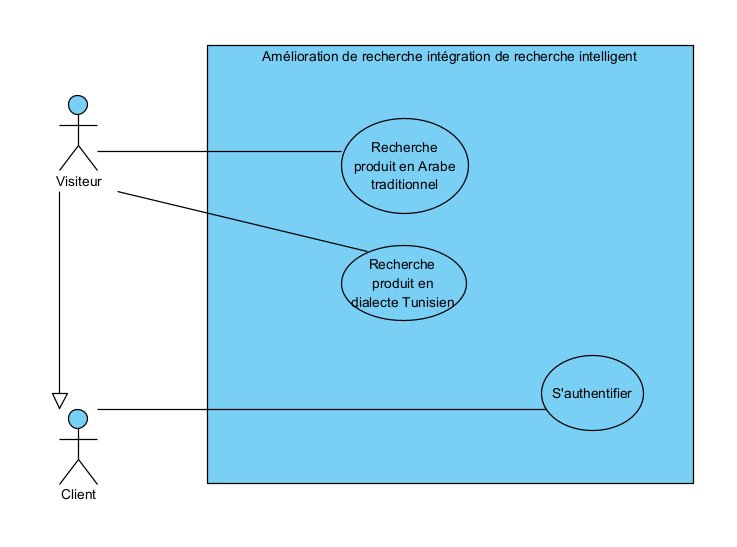
\includegraphics[width=1\textwidth]{logos/cusprint2.png}
	\caption{Diagramme de cas d'utilisation générale du Sprint 2}
	\label{fig:recherchearabe}
\end{figure}

\section{Description textuelle des cas d’utilisations}
Une fois les divers cas d'utilisation présentés, nous examinerons de plus près certains
d'entre eux en fournissant la description textuelle de certains d'entre eux.

\newpage
\subsection{Description textuelle du CU « Rechercher produit en arabe traditionnel »}
\noindent
\textbf{Titre:} Rechercher produit en arabe traditionnel \\
\textbf{Résumé:} Le client saisit son terme de recherche en arabe traditionnel, en cliquant sur le boutton pour rechercher le(s) produit(s) qu'il veut chercher. \\
\textbf{Acteur Principal:} Client \\
\textbf{Précondition:} \begin{enumerate}
	\item Le client (ou le visiteur) est sur la page de recherche
	\item Le client (ou le visiteur) a saisi son terme de recherche en arabe traditionnel
	\item Le client (ou le visiteur) a cliqué sur "Rechercher"
\end{enumerate}
\textbf{Postcondition:} Le(s) produit(s) que le client (ou le visiteur) cherche est renvoyé, s'il n'existe pas, le systéme renvoie des produits similaires comme suggestion. \\
\textbf{Scénario de base: }
\begin{enumerate}
	\item Le client saisit son terme de recherche.
	\item Le client clique sur le boutton "Rechercher"
	\item Le système prend le terme de recherche, en vérifiant que c'est en arabe traditionnel, et le traduit en français.
	\item Le système prend ce terme de recherche, et performe les étapes nécessaires pour la convertir en vecteur.
	\item Le système compare ce vecteur contre les vecteurs dans Elasticsearch.
	\item Le système renvoie les produits.
\end{enumerate}

\newpage
\textbf{Scénario alternatifs : }
\begin{enumerate}
	\item Le terme de recherche est vide:
	      \begin{enumerate}
		      \item Le système affiche un message d'erreur informant le client que le terme de recherche est requis.
		      \item Retour à l'étape 1 du scénario de base.
	      \end{enumerate}
	\item Le terme de recherche n'est pas en arabe traditionnel:
	      \begin{enumerate}
		      \item Le système suppose que le terme recherché est en drançais.
		      \item Passer à la 4ème étape des scénarios de base.
	      \end{enumerate}
	\item Le(s) produit(s) que le client cherche n'existe pas.
	      \begin{enumerate}
		      \item Le système essaie de renvoyer les produits les plus similaires comme des suggestions.
		      \item Retour à l'étape 1 du scénario de base.
	      \end{enumerate}
\end{enumerate}

\subsection{Description textuelle du CU « Rechercher produit en arabe en dialecte tunisien »}
\noindent
\textbf{Titre:} Rechercher produit en arabe en dialecte tunisien \\
\textbf{Résumé:} Le client(ou le visiteur) saisit son terme de recherche en arabe en dialecte tunisien, en cliquant sur le boutton pour rechercher le(s) produit(s) qu'il veut chercher. \\
\textbf{Acteur Principal:} Client \\
\textbf{Précondition:} \begin{enumerate}
	\item Le client (ou le visiteur) est sur la page de recherche
	\item Le client (ou le visiteur) a saisi son terme de recherche en arabe en dialecte tunisien
	\item Le client (ou le visiteur) a cliqué sur "Rechercher"
\end{enumerate}
\textbf{Postcondition:} Le(s) produit(s) que le client cherche est renvoyé, s'il n'existe pas, le système renvoie des produits similaires comme suggestion. \\
\textbf{Scénario de base: }
\begin{enumerate}
	\item Le client saisit son terme de recherche en arabe en dialecte tunisien.
	\item Le client clique sur la boutton "Rechercher"
	\item Le système prend le terme de recherche, en vérifiant que c'est en arabe en dialecte Tunisien, et le traduit en Français.
	\item Le système prend ce terme de recherche, et performe les étapes nécessaires pour la convertir en vecteur.
	\item Le système compare ce vecteur contre les vecteurs dans Elasticsearch.
	\item Le système renvoie les produits.
\end{enumerate}

\textbf{Scénario alternatifs : }
\begin{enumerate}
	\item Le terme de recherche est vide:
	      \begin{enumerate}
		      \item Le système affiche un message d'erreur informant le client que le terme de recherche est requis.
		      \item Retour à l'étape 1 du scénario de base.
	      \end{enumerate}
	\item Le terme de recherche n'est pas en arabe en dialecte tunisien:
	      \begin{enumerate}
		      \item Le système suppose que le terme recherché est en français.
		      \item Passer à la 4ème étape des scénarios de base.
	      \end{enumerate}

	\item Le(s) produit(s) que le client cherche n'existe pas.
	      \begin{enumerate}
		      \item Le système essaie de renvoyer les produits les plus similaires comme des suggestions.
		      \item Retour à l'étape 1 du scénario de base.
	      \end{enumerate}
\end{enumerate}

\subsection{Description textuelle du CU << Voir suggestions >>}
\noindent
\textbf{Titre:} Voir suggestions \\
\textbf{Résumé:} Après la recherche du produit, le systéme essaie de suggérer au client des produits similaires. \\
\textbf{Acteur Principal:} Client \\
\textbf{Précondition:} \begin{enumerate}
	\item Le client est authentifié.
	\item Le client a déja cherché un produit.
\end{enumerate}
\textbf{Postcondition:} Le(s) produit(s) que le client cherche est renvoyé, et le systéme renvoie des produits similaires comme suggestions. \\
\textbf{Scénario de base: }
\begin{enumerate}
	\item Le client cherche un produit.
	\item Le système cherche le produit.
	\item Le système renvoie les produits ainsi que des suggestions des produits similaires.
\end{enumerate}

\textbf{Scénario alternatifs : }
\begin{enumerate}
	\item Le(s) produit(s) que le client cherche n'existe pas.
	      \begin{enumerate}
		      \item Le système essaie de renvoyer les produits les plus similaires comme des suggestions.
		      \item Retour à l'étape 1 du scénario de base.
	      \end{enumerate}
\end{enumerate}